\documentclass[journal]{vgtc}                      % final (journal style)
%\documentclass[review,journal]{vgtc}              % review (journal style)
%\documentclass[widereview]{vgtc}                  % wide-spaced review
%\documentclass[preprint,journal]{vgtc}            % preprint (journal style)

\onlineid{0}

%% Declare the category of your paper, only shown in review mode
\vgtccategory{Research}

%% Remove the IEEE "Manuscript received ..." / reprints / DOI note from the first page.
\manuscriptnote{}

%% Paper title.
\title{Visualizing Patient Flows in Brazil's Unified Health System: An Interactive Map of {SIH/SUS} Hospitalizations}

%% Author names and affiliations. Replace the placeholder names and e-mails.
\author{%
  Arthur Sudbrack Ibarra,
  Delmar Lucas Dorneles Quaresma,
  Eduardo Villarinho Curia\\
  Kelvin Queiros Pessoa,
  and Lucas Angelo Loges%
}

\authorfooter{
  \item
  	All authors are with the Pontifical Catholic University of Rio Grande do Sul (PUCRS), Porto Alegre, Brazil.
  	E-mail: arthur.ibarra@edu.pucrs.br, delmar.q91@edu.pucrs.br, eduardo.curia@edu.pucrs.br, kelvin.pessoa@edu.pucrs.br, lucas.loges@edu.pucrs.br.
}

%% Abstract section.
\abstract{
  Brazil's Unified Health System (SUS) records every publicly funded hospital admission in the SIH/SUS dataset, a general-purpose source that also stores the patient's municipality of residence and the municipality where the admission took place.
  Together these two fields describe how patients move across the country to be hospitalized, yet the official tabular access hides this movement and can conceal where a region depends on outside care.
  We present an interactive flow map that draws these movements as origin-destination arcs over a map of Brazil.
  The view is organized in three levels, country, state, and city, and supports filtering by medical specialty, year, and month, along with side panels that rank attracting and dependent municipalities and compare resident and incoming admissions across the year.
  Using 183 million admissions from 2008 to 2023, we present case studies that illustrate how the tool is designed to surface care gaps, regional hubs, and seasonal patterns that tabular access tends to obscure.
  This paper describes the design and the system; an evaluation with users remains future work.%
}

%% Keywords that describe your work. Will show as 'Index Terms' in journal
\keywords{Geographic visualization, flow maps, origin-destination data, public health, interactive visualization.}

%% Uncomment and add a teaser image once one is available.
%\teaser{
%  \centering
%  \includegraphics[width=\linewidth]{teaser}
%  \caption{The interactive flow map at the national level.}
%  \label{fig:teaser}
%}

%%%%%%%%%%%%%%%%%%%%%%%%%%%%%%%%%%%%%%%%%%%%%%%%%%%%%%%%%%%%%%%%
%%%%%%%%%%%%%%%%%%%%%% LOAD PACKAGES %%%%%%%%%%%%%%%%%%%%%%%%%%%
%%%%%%%%%%%%%%%%%%%%%%%%%%%%%%%%%%%%%%%%%%%%%%%%%%%%%%%%%%%%%%%%

\graphicspath{{figs/}{figures/}{pictures/}{images/}{./}}

\usepackage{booktabs}                  % for tables
\usepackage{mathptmx}                  % use matching math font
\usepackage{graphicx}                  % for figures
\usepackage{tikz}                      % for the architecture diagram
\usetikzlibrary{arrows.meta,positioning}

\begin{document}

%%%%%%%%%%%%%%%%%%%%%%%%%%%%%%%%%%%%%%%%%%%%%%%%%%%%%%%%%%%%%%%%
%%%%%%%%%%%%%%%%%%%%%% START OF THE PAPER %%%%%%%%%%%%%%%%%%%%%%
%%%%%%%%%%%%%%%%%%%%%%%%%%%%%%%%%%%%%%%%%%%%%%%%%%%%%%%%%%%%%%%%

\firstsection{Introduction}

\maketitle

Brazil's Unified Health System (SUS) gives every resident the right to public hospital care.
In practice, hospitals and medical specialties are spread unevenly across the country, so many patients leave their home town to be admitted elsewhere.
Knowing where these patients go, and for which specialties, helps managers plan hospital beds and find regions that depend on care produced somewhere else.

The Hospital Information System of SUS (SIH/SUS), published by DATASUS, records every publicly funded hospital admission.
Each record stores the patient's municipality of residence and the municipality of the hospital, so a single admission already describes a movement between two places.
The data is large: our extract holds more than 180 million admissions from 2008 to 2023.
At this size, tables and static maps make it hard to see the overall pattern of movement between cities and states.

We present an interactive flow map of these hospitalization flows.
Each arc links the patient's residence to the hospital municipality, and its width grows with the number of admissions.
The map works at three levels, from the whole country down to one state and then one city, so the user opens detail only where it is needed.
Filters by medical specialty, year range, and month narrow the data, and a side panel ranks the cities that most attract patients and the ones whose residents most depend on care elsewhere.

The design answers four questions raised in the first part of this work:
(1) what share of patients is treated outside their home municipality, and how it varies by specialty;
(2) where the care gaps are for specific specialties such as oncology;
(3) which cities sustain the hospital care of a whole region;
and (4) whether seasonal peaks in admissions are driven by patients coming from outside.
This paper describes how we prepared the data and designed the visualization, and shows how it answers these questions for admissions between 2008 and 2023.

\section{Related Work}

Several studies use SIH/SUS data to study where Brazilians are hospitalized.
Oliveira et al.~\cite{Oliveira2004TerritoriosSistema} mapped hospital care networks and found that most admissions still happen in the patient's own municipality, while the remaining flows point toward regional hubs.
Rocha et al.~\cite{Rocha2015HospitalizationFlow} measured patient migration between health regions in S\~{a}o Paulo and classified each region as attracting or losing patients.
Xavier et al.~\cite{Xavier2019RegioesSaude} used the origin and destination of admissions to build health regions and to locate care gaps.
These works report indices, tables, and static maps, but they rarely let the reader explore the flows directly.

Information visualization has long studied how to draw origin-destination (OD) data.
Drawing every flow as a straight line produces heavy occlusion, so much of the work looks for ways to reduce clutter.
Wood et al.~\cite{Wood2010VisualisationOrigins} replaced lines with small gridded maps (OD maps) to avoid crossing flows, while Jenny et al.~\cite{Jenny2018DesignPrinciples} proposed design principles for line-based flow maps and Graser et al.~\cite{Graser2019Untangling} compared techniques for untangling OD flows in a GIS.
For data that changes over time, Flowstrates~\cite{Boyandin2011Flowstrates} separates origins, destinations, and a temporal heatmap.
We borrow the clutter-reduction goal from this line of work and apply it through three concrete choices: curved arcs in place of straight lines, aggregation by administrative level so that only a tractable number of arcs is drawn at once, and a direction filter that hides the arcs the user is not inspecting.

Interaction is what lets users work with large and multivariate data.
Shneiderman's mantra of overview first, zoom and filter, then details on demand~\cite{Shneiderman1996EyesHaveIt}, together with the interaction categories of Yi et al.~\cite{Yi2007TowardDeeper}, describes the operations our tool depends on.
The three-level drill-down and the specialty and time filters put these ideas to work on the hospitalization data.

General flow-map tools such as kepler.gl and flowmap.blue can plot OD data, but they are generic plotters that a user must configure for each dataset.
Our work connects the two threads above and adds three features that a generic plotter does not provide on this data.
First, a three-level drill-down bound to the Brazilian administrative hierarchy, from federative unit to municipality.
Second, a precomputed aggregation that keeps the full 183 million record dataset interactive.
Third, panels built for the access questions at hand: an attraction ranking and a resident-versus-incoming seasonal comparison.


\section{Proposed Visualization}

\subsection{Data preparation}

The raw SIH/SUS extract is too large to query while the user waits.
It holds about 183 million admissions in a 26\,GB table, and a single aggregation over one year already takes tens of seconds.
To keep the interface responsive, we move all of the heavy work to an offline step that runs once.

This step makes one pass over the fact table.
It joins each admission to the municipality where the patient lives and to the municipality of the hospital, then groups the rows by origin, destination, specialty, year, and month.
The result is a small set of tables, the largest with 13.5 million rows, that the application reads in place of the raw data.
Figure~\ref{fig:architecture} shows this pipeline.
Queries against these tables return in under 100 milliseconds, so filtering and navigation feel immediate.

\begin{figure}[t]
  \centering
  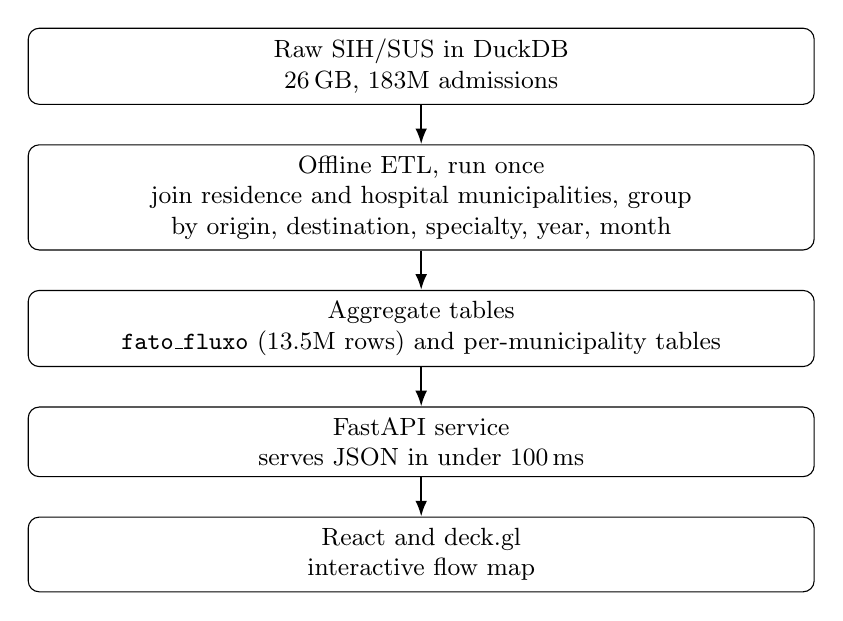
\begin{tikzpicture}[
    node distance=5mm,
    box/.style={draw, rounded corners, align=center, inner sep=4pt,
                font=\small, text width=0.80\columnwidth},
    arr/.style={-{Latex[length=2mm]}, thick}
  ]
    \node[box] (raw)  {Raw SIH/SUS in DuckDB\\26\,GB, 183M admissions};
    \node[box, below=of raw]  (etl)  {Offline ETL, run once\\join residence and hospital municipalities, group by origin, destination, specialty, year, month};
    \node[box, below=of etl]  (agg)  {Aggregate tables\\\texttt{fato\_fluxo} (13.5M rows) and per-municipality tables};
    \node[box, below=of agg]  (api)  {FastAPI service\\serves JSON in under 100\,ms};
    \node[box, below=of api]  (front){React and deck.gl\\interactive flow map};
    \draw[arr] (raw)  -- (etl);
    \draw[arr] (etl)  -- (agg);
    \draw[arr] (agg)  -- (api);
    \draw[arr] (api)  -- (front);
  \end{tikzpicture}
  \caption{%
    Data pipeline.
    All aggregation runs once, offline, turning the 183 million row table into small tables that the service can query in under 100 milliseconds.%
  }
  \label{fig:architecture}
\end{figure}

\subsection{The flow map}

We draw each hospitalization flow as a curved arc from the patient's residence to the hospital municipality.
The width of the arc grows with the number of admissions, so the thickest arcs mark the busiest routes.
Color marks the direction relative to the place in focus, with arcs that leave a region drawn in orange and arcs that arrive drawn in blue.

A choropleth sits behind the arcs and fills each state or city with one chosen metric.
The default metric is the attraction balance, the number of admissions a place receives minus the number its own residents generate.
Blue means the place treats more patients than it sends away, and red means the opposite.
City nodes appear as circles sized by the number of admissions that pass through them.
A dark basemap keeps the arcs and nodes easy to read.

\subsection{Three levels of detail}

The map follows the principle of overview first, then zoom and filter, then details on demand~\cite{Shneiderman1996EyesHaveIt}.
It opens at the national level, where the 27 states are the nodes and the arcs show flows between states.
Clicking a state opens the state level, where its municipalities become the nodes and the arcs show flows inside the state and toward other states.
Clicking a city opens the city level, which shows every flow that touches that city across the country.
Figure~\ref{fig:drilldown} shows the three levels for Rio Grande do Sul.
A breadcrumb at the top records the path and lets the user step back, and the camera flies to each new selection.

\begin{figure}[t]
  \centering
  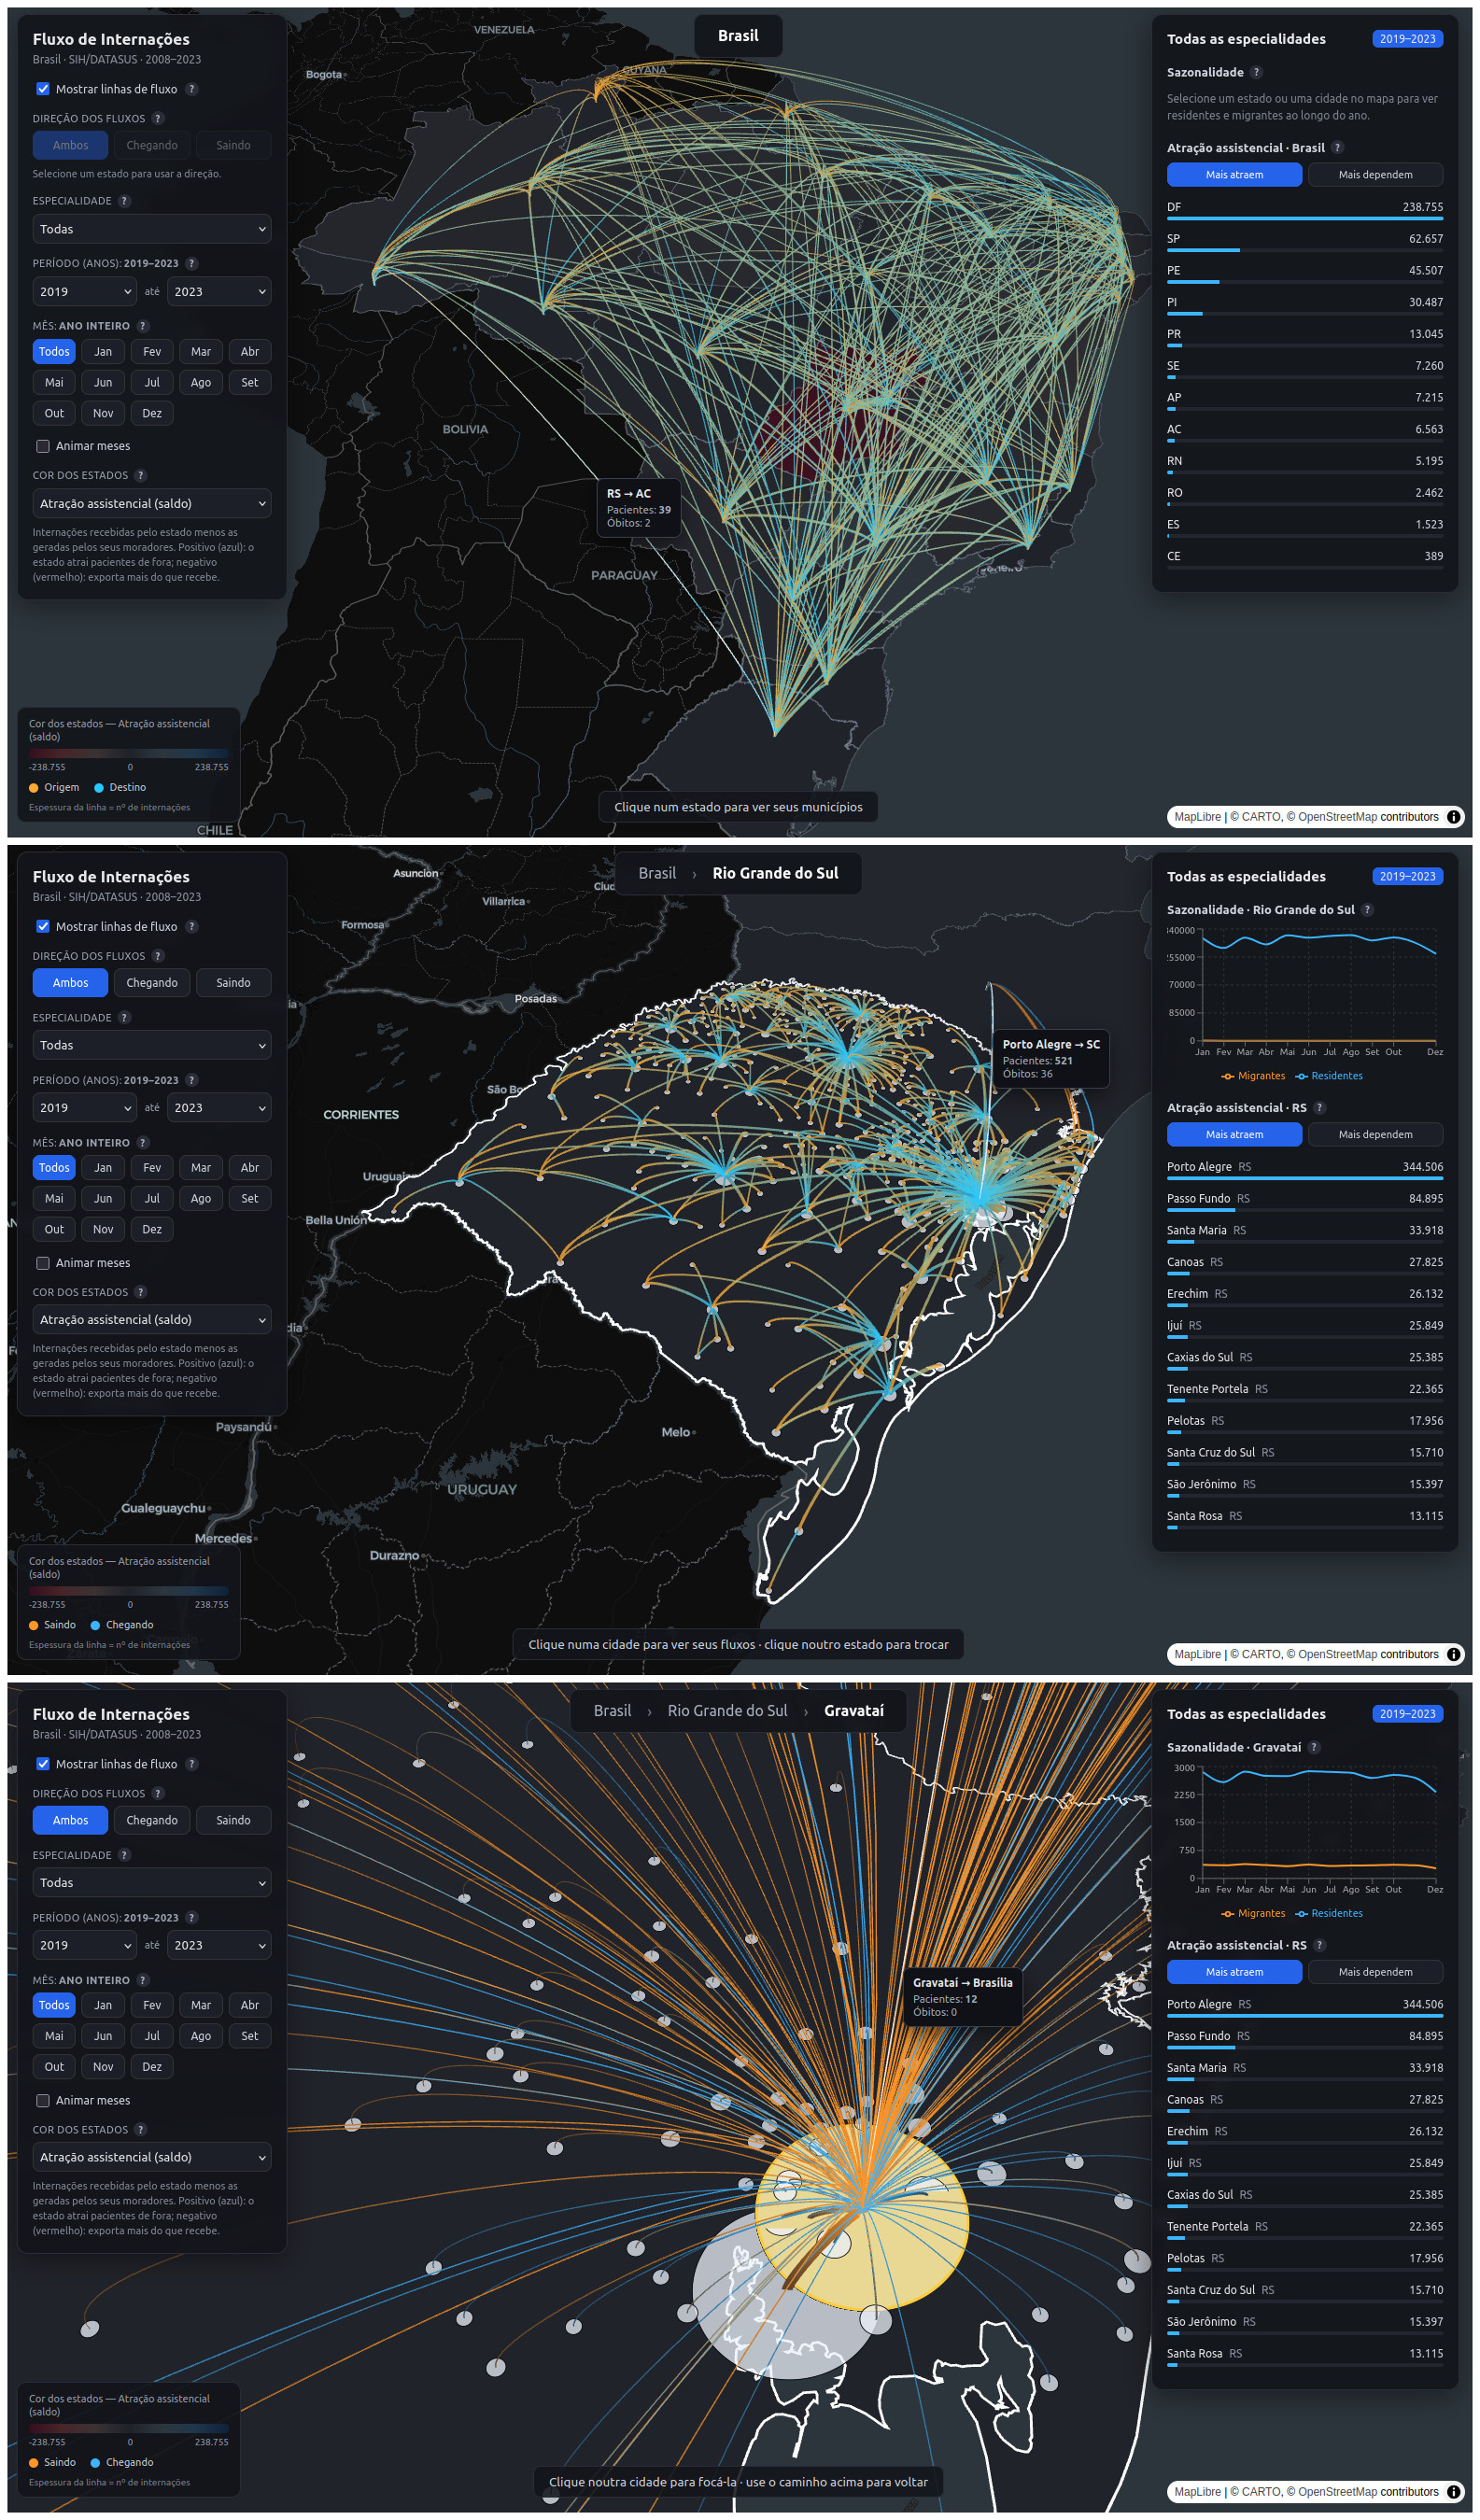
\includegraphics[width=0.78\columnwidth]{national-to-city-view.jpeg}
  \caption{%
    The three levels of the flow map for Rio Grande do Sul.
    Top: the national level, with states as nodes and arcs between them.
    Middle: the state level, with municipalities as nodes.
    Bottom: the city level, showing every flow that touches the selected city.%
  }
  \label{fig:drilldown}
\end{figure}

\subsection{Filters and animation}

Filters narrow the data without leaving the map.
The user can pick a medical specialty, a range of years, and a single month, and can change the metric used for the choropleth.
A direction control limits the arcs to those leaving or arriving at the focus, which removes clutter when a city has many connections.
A further option plays the twelve months in sequence, so seasonal change appears as motion on the map.

\subsection{Analytical panels}

Two side panels turn the map into direct answers.
The ranking panel lists the places with the strongest attraction balance, and a toggle switches between the cities that attract the most patients and the cities that most depend on others.
Figure~\ref{fig:ranking} shows this ranking for Rio Grande do Sul, with Porto Alegre as the clear hub and Viam\~{a}o among the most dependent municipalities.

The second panel plots a monthly time series that separates resident admissions from incoming ones.
This shows whether a seasonal peak comes from local patients or from people arriving from elsewhere.

The arc colors make the same contrast visible on the map.
Figure~\ref{fig:contrast} compares the two municipalities from the ranking, filtered to facial surgery between 2015 and 2023.
Porto Alegre is covered by blue arcs that arrive from across the state and from other states, while Viam\~{a}o shows mostly orange arcs that leave for nearby cities.

\begin{figure}[t]
  \centering
  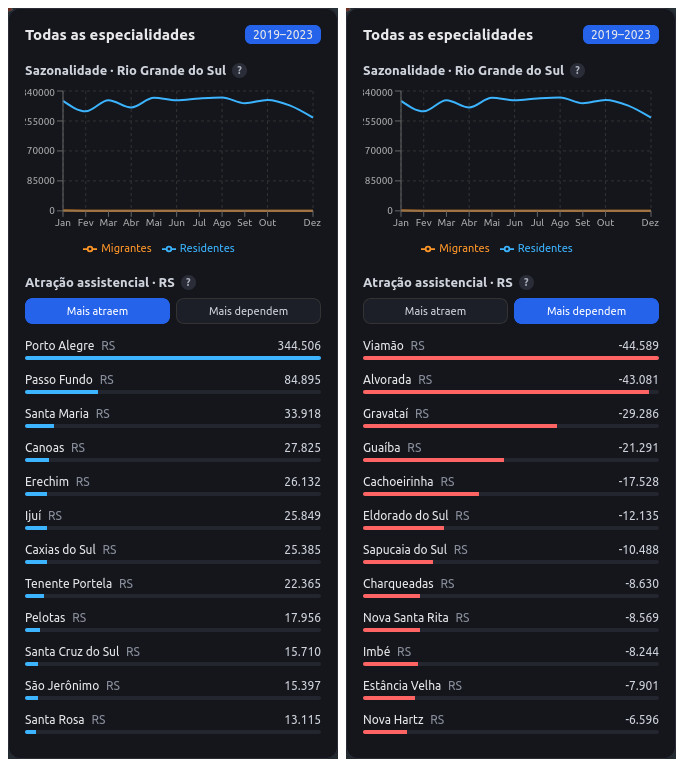
\includegraphics[width=0.92\columnwidth]{attract-vs-depend-more.jpeg}
  \caption{%
    The attraction ranking for Rio Grande do Sul, all specialties, 2019 to 2023.
    Left: the municipalities that attract the most patients, led by Porto Alegre.
    Right: the municipalities that most depend on care elsewhere, led by Viam\~{a}o.
    Bar length encodes the attraction balance, blue for positive and red for negative.%
  }
  \label{fig:ranking}
\end{figure}

\begin{figure}[t]
  \centering
  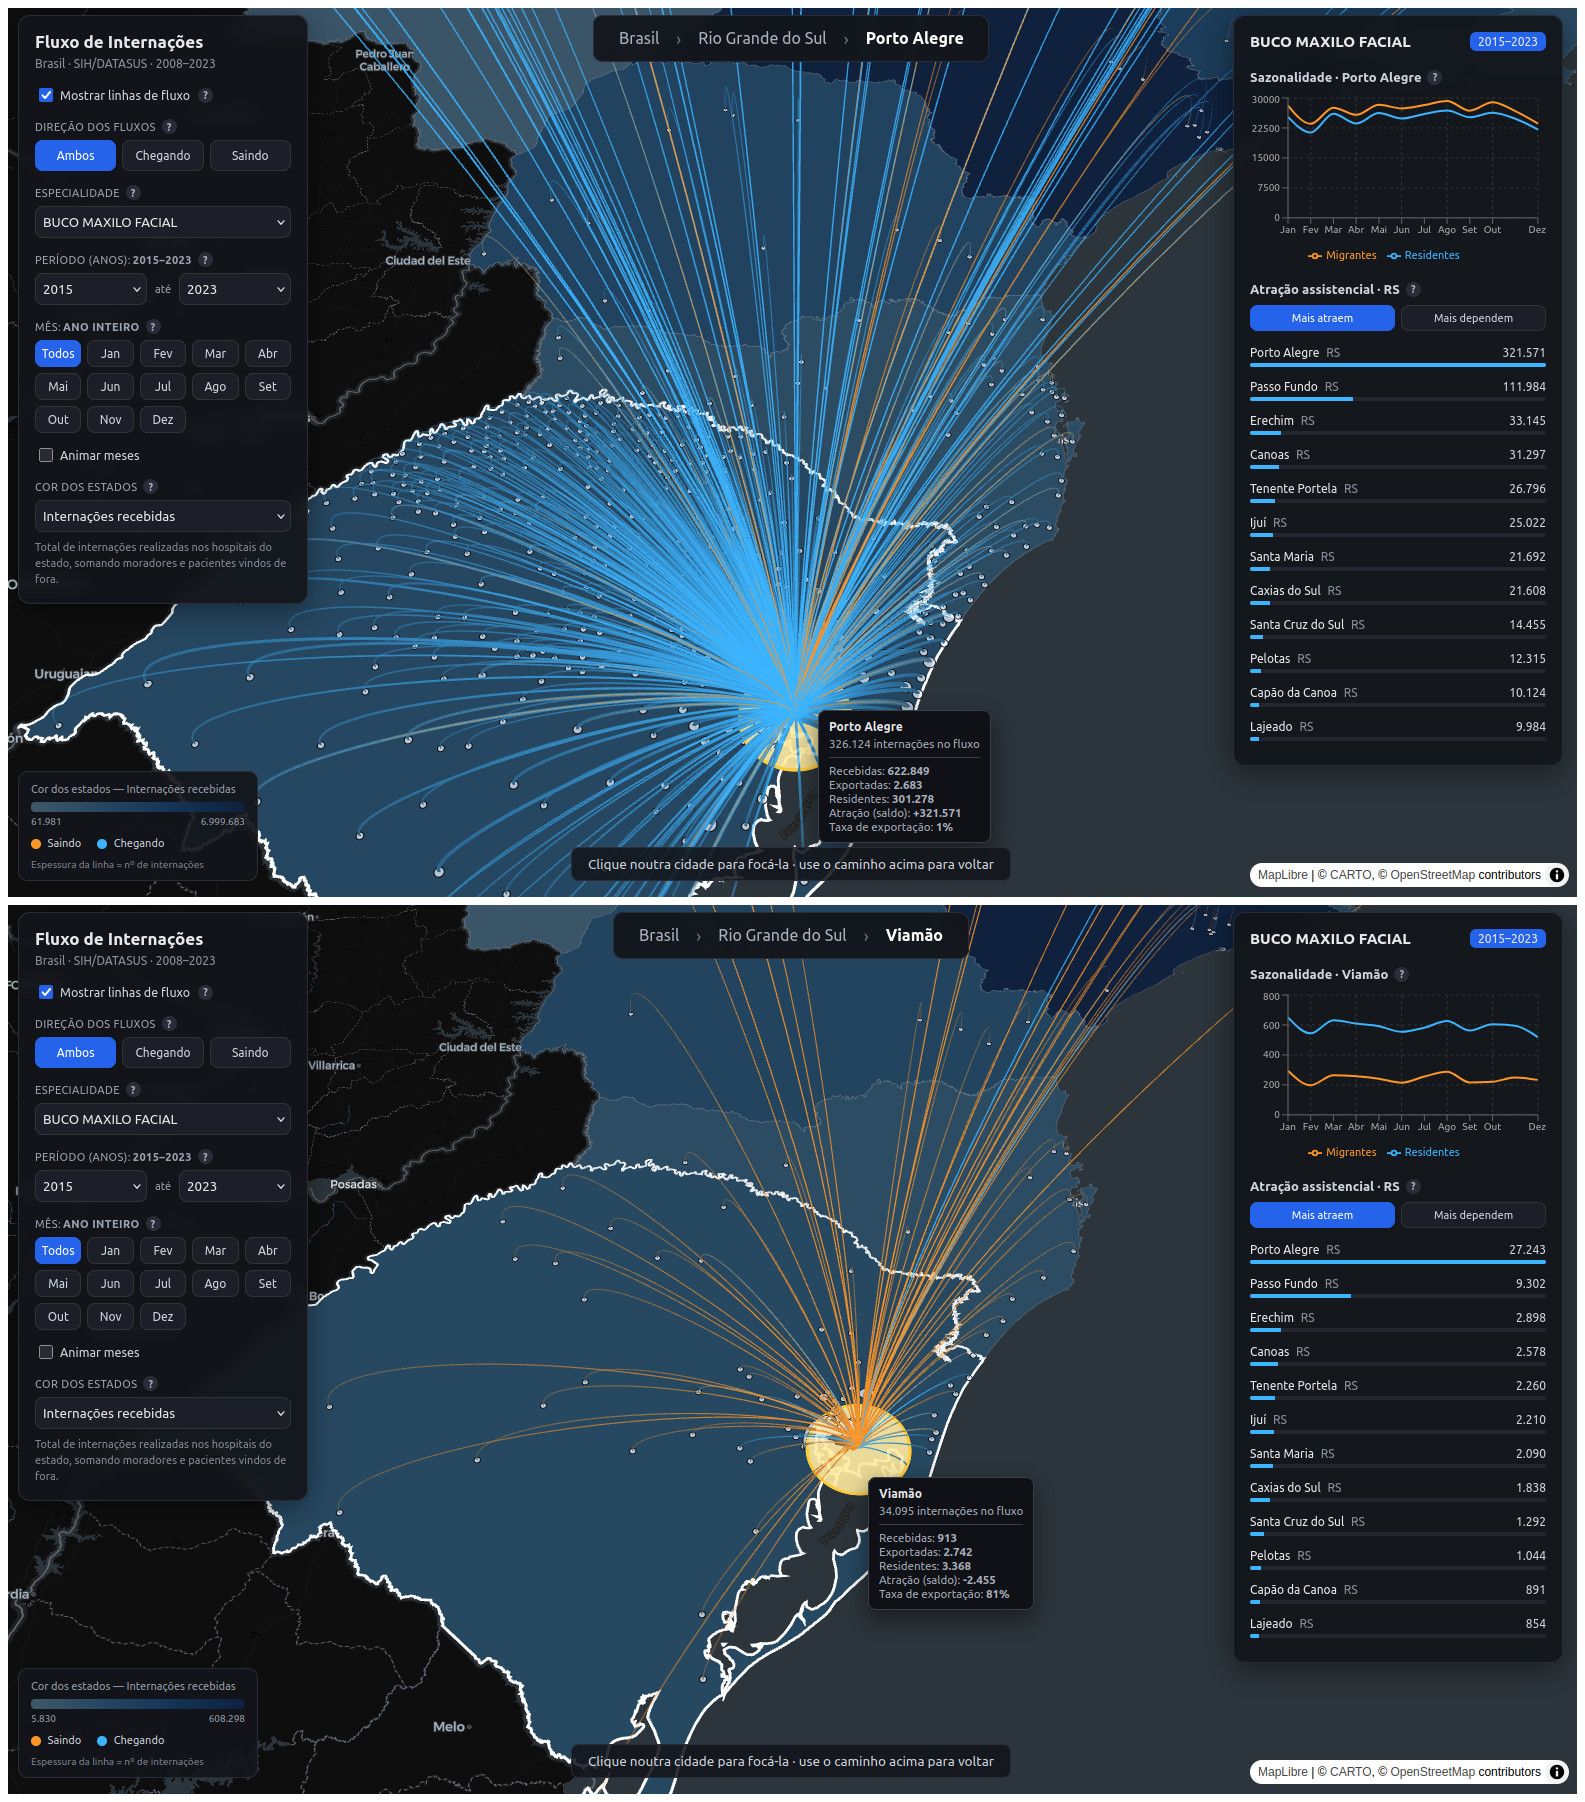
\includegraphics[width=0.92\columnwidth]{poa-vs-viamao-buco-maxilo-facial.jpeg}
  \caption{%
    City level view of two municipalities in Rio Grande do Sul for facial surgery (Buco Maxilo Facial), 2015 to 2023.
    Porto Alegre (top) is reached by many blue arcs, since patients arrive from across the state and from other states.
    Viam\~{a}o (bottom) shows mostly orange arcs, since its residents leave for other cities.
    The two were the top attracting and top dependent municipalities in the ranking of Figure~\ref{fig:ranking}.%
  }
  \label{fig:contrast}
\end{figure}

\section{Analysis of Results}

We now apply the tool to the three themes set out in the Introduction.
The aim is not a complete study of any theme, but a demonstration that the visualization can surface the relevant patterns, which tabular access tends to obscure.
Each example uses complete years, since the latest year in the extract still lacks part of its final months.
As a general figure, close to 34 percent of admissions between 2015 and 2019 took place outside the patient's home municipality, so cross-border flow is substantial and worth visualizing.

\subsection{Gaps in care for a specialty}

The first theme is the gap in care, where the residents of a region must travel for a given specialty.
A municipality can be a hub for one specialty and dependent for another.
Figure~\ref{fig:gap} shows Santa Maria, a hub in the interior of Rio Grande do Sul, under two specialties in 2023.
For cardiology it received 3{,}391 admissions against 2{,}061 from its own residents, a positive balance of 1{,}330 and an export rate of 1 percent.
For gastroenterology it received 281 against 405 residents, a negative balance of 124 and an export rate of 45 percent.

Changing only the specialty filter turns Santa Maria from a blue hub reached by incoming arcs into a red municipality whose residents leave for other cities.
A pattern of this kind points a health authority to a specialty and a region that may need attention.
Because the coverage of the specialty field is uneven, the reading is most reliable where a specialty has many admissions.

\subsection{Hub cities and regional load}

The second theme is the hub city that concentrates the care of a region, where the demand it absorbs may signal overload or a bottleneck.
The ranking panel orders municipalities by their attraction balance.
Figure~\ref{fig:ranking} shows Rio Grande do Sul, where Porto Alegre attracts far more patients than any other city, followed by Passo Fundo and Santa Maria, while Viam\~{a}o, Alvorada, and Gravata\'{\i} appear among the municipalities that depend on care produced elsewhere.
A small number of hubs therefore sustains many surrounding towns.

The map shows the same balance for a single specialty.
Figure~\ref{fig:contrast} draws facial surgery for the two extremes of the ranking.
Porto Alegre is covered by incoming blue arcs from across the state and from other states, whereas Viam\~{a}o shows mostly outgoing orange arcs.
The width and direction of the arcs report the export of patients for the chosen specialty.
The per-capita metric helps separate a large hub from one that is heavily loaded for its population, which is where a bottleneck is most likely.

\subsection{Seasonal patterns}

The third theme is seasonality, and whether a peak month falls on residents or on incoming patients.
The monthly balance proves specific to each city.
Figure~\ref{fig:seasonality} shows six municipalities across the twelve months of 2021.
Vit\'{o}ria da Conquista (BA) is the most common case, where residents and incoming patients rise and fall together.
Cear\'{a}-Mirim (RN) shows both groups climbing sharply from March, a clear peak that a hospital could anticipate.

The other four cities show patterns that do not generalize.
In Muri\'{a}e (MG) the incoming patients peak several times while residents stay flat.
In Gurupi (TO) the resident and incoming peaks alternate through the year.
In Luzi\^{a}nia (GO) and Teut\^{o}nia (RS) a rise in residents coincides with a fall in incoming patients, which suggests that residents are served first when local demand grows; Teut\^{o}nia also peaks in winter.

This bears on the question of overload in peak months.
In most cities residents and incoming patients move together, so a peak is not driven by a sudden influx from outside.
In the few cities where the two diverge, the system appears to favor residents during the busiest months.
Because the behavior varies so widely, the practical value of the monthly view is local: an institution can read the curve for its own city and prepare for its own peak.

\begin{figure}[t]
  \centering
  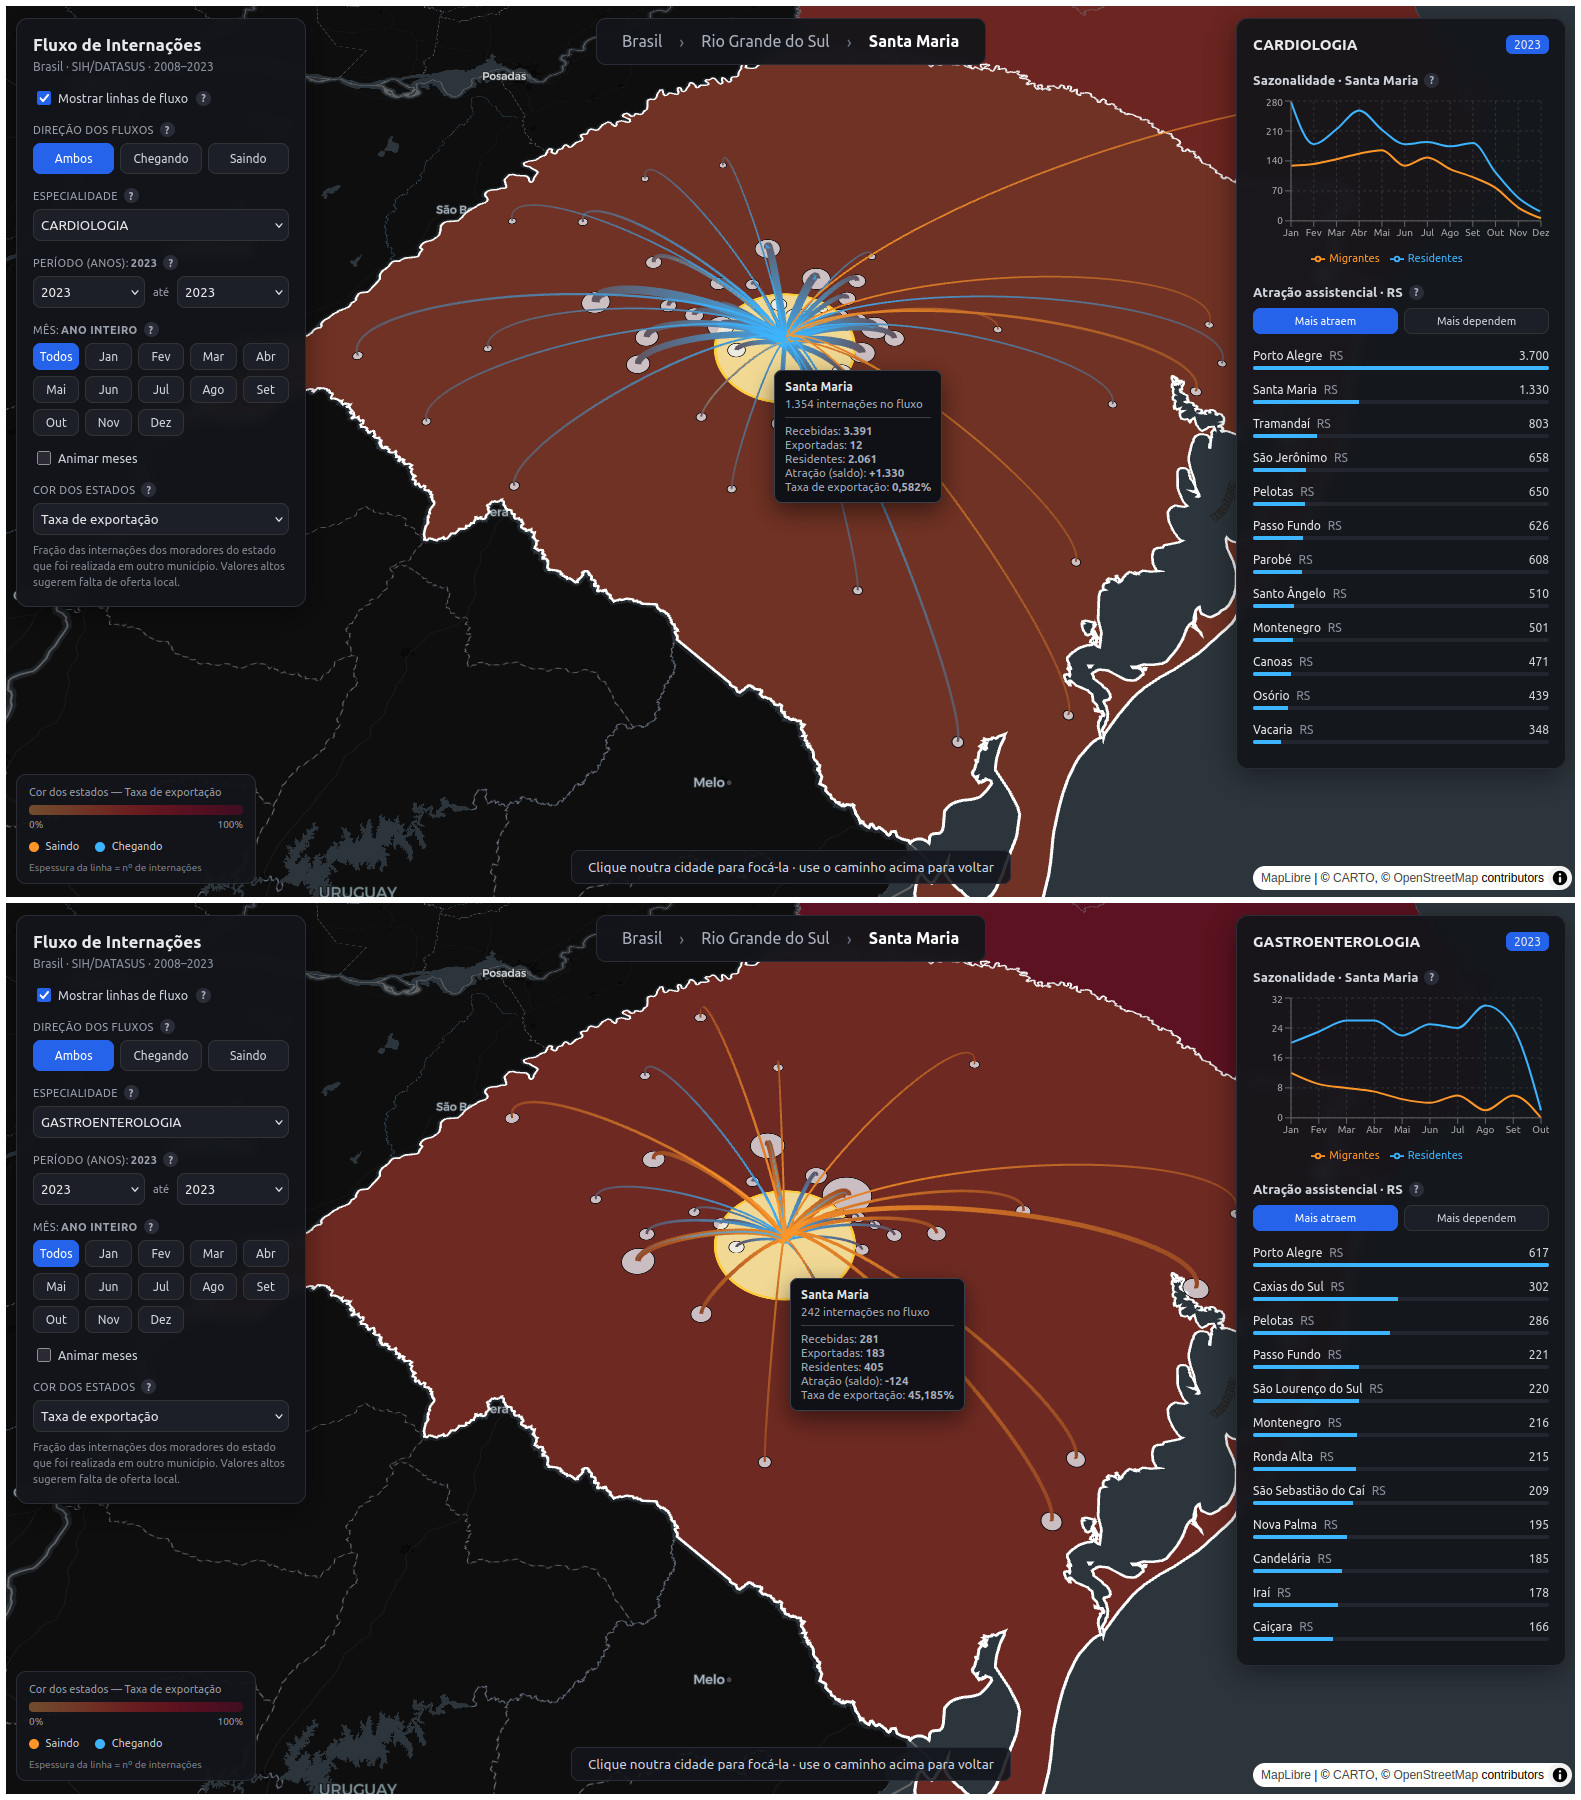
\includegraphics[width=0.95\columnwidth]{santa-maria-cardio-vs-gastro.jpeg}
  \caption{%
    Santa Maria (Rio Grande do Sul) under two specialties in 2023.
    Top: cardiology, where the city is a hub reached by incoming blue arcs (balance $+1{,}330$, export rate 1 percent).
    Bottom: gastroenterology, where its residents leave along orange arcs (balance $-124$, export rate 45 percent).
    Only the specialty filter changed between the two views.%
  }
  \label{fig:gap}
\end{figure}

\begin{figure}[t]
  \centering
  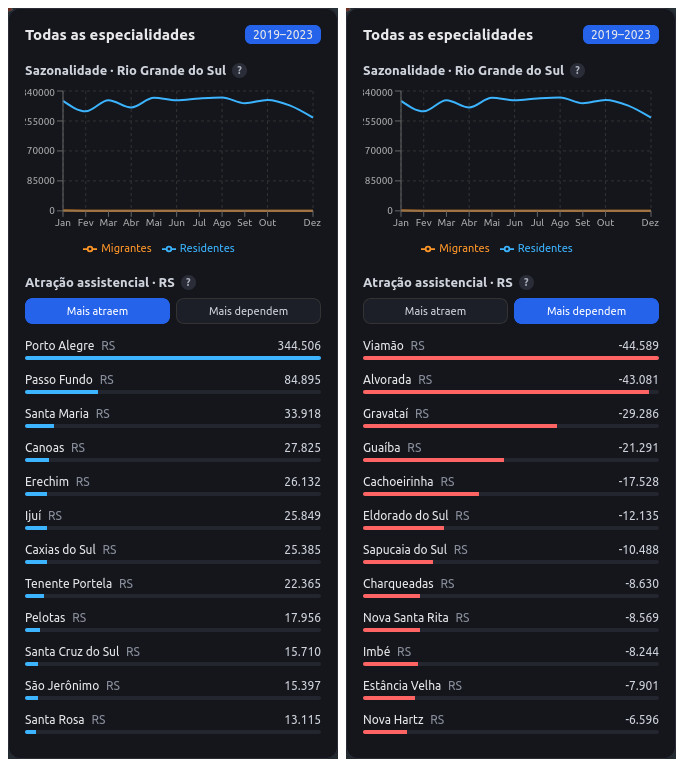
\includegraphics[width=0.92\columnwidth]{attract-vs-depend-more.jpeg}
  \caption{%
    The attraction ranking for Rio Grande do Sul, all specialties, 2019 to 2023.
    Left: the municipalities that attract the most patients, led by Porto Alegre.
    Right: the municipalities that most depend on care elsewhere, led by Viam\~{a}o.
    Bar length encodes the attraction balance, blue for positive and red for negative.%
  }
  \label{fig:ranking}
\end{figure}

\begin{figure}[t]
  \centering
  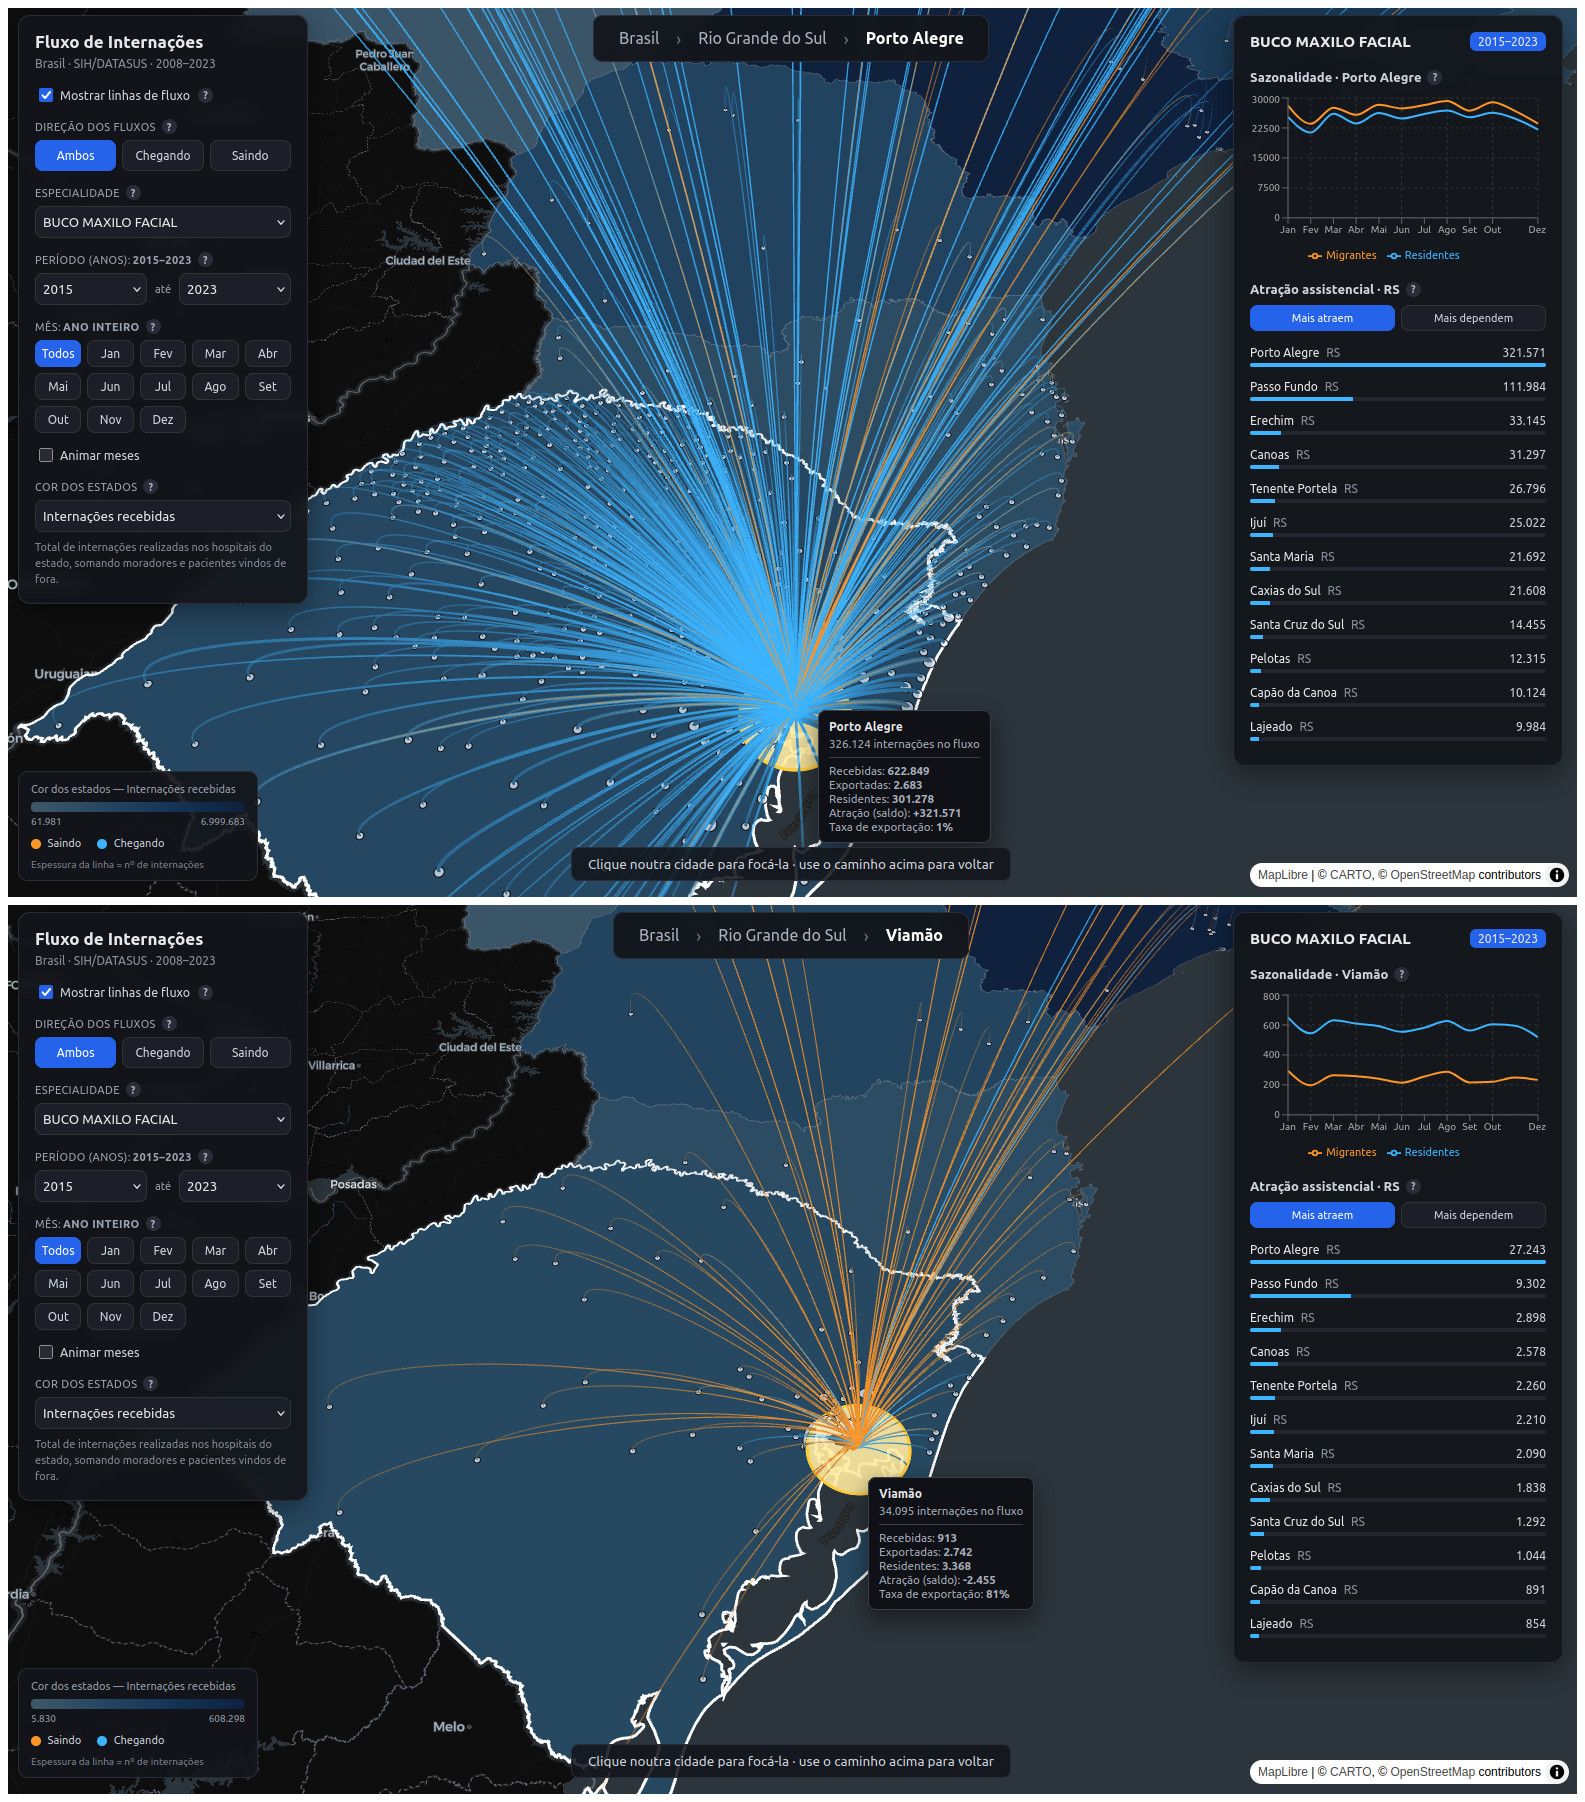
\includegraphics[width=0.92\columnwidth]{poa-vs-viamao-buco-maxilo-facial.jpeg}
  \caption{%
    City level view of two municipalities in Rio Grande do Sul for facial surgery (Buco Maxilo Facial), 2015 to 2023.
    Porto Alegre (top) is reached by many blue arcs, since patients arrive from across the state and from other states.
    Viam\~{a}o (bottom) shows mostly orange arcs, since its residents leave for other cities.
    The two are the top attracting and top dependent municipalities in the ranking of Figure~\ref{fig:ranking}.%
  }
  \label{fig:contrast}
\end{figure}

\begin{figure*}[t]
  \centering
  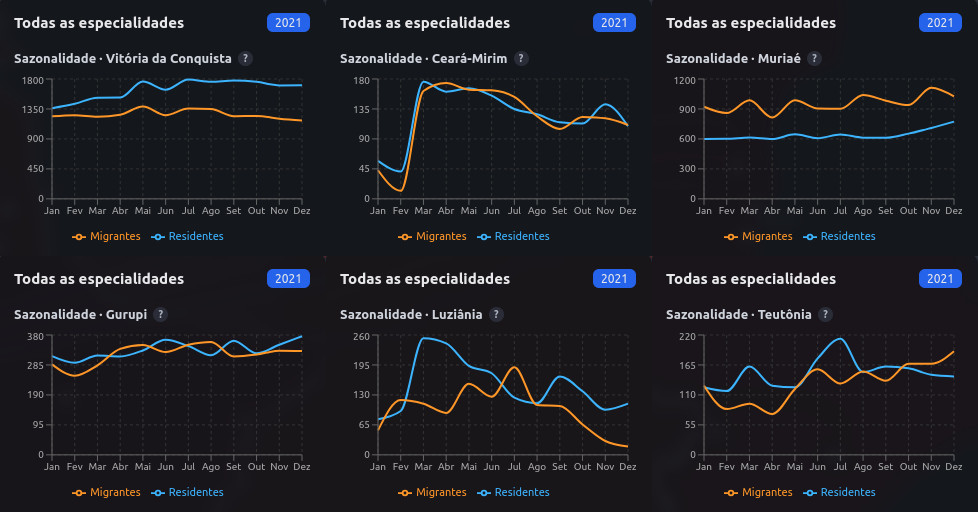
\includegraphics[width=\linewidth]{seasonal-charts.jpeg}
  \caption{%
    Monthly resident and incoming admissions for six municipalities in 2021.
    The shape of the curve changes from city to city, from residents and incoming patients moving together (Vit\'{o}ria da Conquista, BA) to shared peaks (Cear\'{a}-Mirim, RN), repeated incoming peaks (Muri\'{a}e, MG), alternating peaks (Gurupi, TO), and resident peaks that coincide with drops in incoming patients (Luzi\^{a}nia, GO and Teut\^{o}nia, RS).%
  }
  \label{fig:seasonality}
\end{figure*}

\section{Conclusion and Future Work}

We presented an interactive flow map of hospital admissions in the Brazilian public system.
The tool draws each admission as an arc from the patient's residence to the hospital municipality, works at the national, state, and municipal levels, and lets the user filter by specialty, year, and month.
Through usage scenarios we illustrated how it can bring out gaps in care for a specialty, the hub cities that concentrate the care of a region, and the seasonal balance between resident and incoming patients.
The contribution is the visualization itself, which is built to expose movement that the official tabular access leaves implicit.

The central limitation is that we have not evaluated the tool with users.
The scenarios in Section~\ref{sec:scenarios} are hand-picked illustrations, so they show that the tool can produce these readings, not that it helps an analyst reach them faster or more reliably than the existing portal.
We therefore make no claim of measured effectiveness, and a study with health managers, outlined below, is the natural next step.

A second limitation concerns the specialty field.
SIH/SUS records the specialty of the hospital bed (\texttt{ESPEC}), as noted in Section~\ref{sec:design}, and this field is sparsely filled.
A few categories, mainly oral and maxillofacial surgery, general surgery, cardiology, and a combined surgical and diagnostic category, account for almost all admissions, while specialties such as oncology and endocrinology appear in very few records, and several others had too little data to keep.
Much of this care is likely registered through the procedure and diagnosis fields rather than the bed specialty, so a filter built on this single field gives only a partial view.

Other limits follow from the same design choices.
The latest year is incomplete in its final months, so the scenarios rely on complete years.
State-level arcs start from state centroids, and the few municipalities without coordinates are left out.
The per-capita metric depends on IBGE population figures and so covers only 2008 to 2021.
Finally, the tool shows where demand concentrates but does not measure hospital capacity, so it points to possible overload rather than confirming it.

Future work follows directly from these limits.
The first priority is the evaluation that this paper lacks.
We plan two lightweight studies: a walkthrough in which a small group of health-data analysts carry out defined tasks with the tool, and a comparison against the DATASUS portal that measures the time to answer a handful of representative questions.
Both are proposed here rather than reported, since we have not yet run them.

The remaining directions address the data limits.
Reading the procedure and diagnosis fields would recover the specialties that the bed-specialty field misses and would widen the analysis of care gaps.
Joining the flows to the number of SUS beds would turn the signal of concentration into a measure of load.
Finer geography, such as health regions and population-weighted centroids, would sharpen the map, and the cost and length-of-stay fields would add a financial and outcome dimension to the movement of patients.

The SIH/SUS data used here is public and distributed by DATASUS.
The source code of the tool is available from the authors on request.


\bibliographystyle{abbrv-doi-hyperref}
\bibliography{references}

\end{document}
